\documentclass{article}
\usepackage[de]{ukon-infie}
\usepackage[utf8]{inputenc}
\usepackage{algorithm2e}
\usepackage{amsmath}
\usepackage{graphicx}
% kann de oder en sein
% kann bubble break, topexercise sein

\Names{Jonas Probst, Simon Giebenhain}
\Lecture[AnaVis]{Analyse und Visualisierung von Informationen}
\Term{WS 2017/18}

\begin{document}
    \begin{ukon-infie}[15.11.17]{3}

        \begin{exercise}[p=9]{PCA}
        	\question{}
        	{
$A \cdot E_1 = 
\left(
	\begin{array}{c}
		5\\
		-8\\
		-32\\
	\end{array}
\right)$,
$A \cdot E_2 = 
\left(
	\begin{array}{c}
		-1\\
		8\\
		2\\
	\end{array}
\right)$,
$A \cdot E_3 = 
\left(
	\begin{array}{c}
		0\\
		1\\
		0\\
	\end{array}
\right)$,
$A \cdot E_4 = 
\left(
	\begin{array}{c}
		10\\
		-8\\
		-20\\
	\end{array}
\right)$\\
It follows that only $E_2$ is a eigenvector of A. The corresponding eigentvalue is 1.
        	}
        	\question{}
        	{
        		\begin{enumerate}
        			\item Only cardinal (that is numeric) data types, because several mathematical operations, such as multiplication , division and addition are necessary.
        			\item One should use a PCA in order to find out which dimensions of the data can be reduced without losing much information. This is especially important if there is a large number of dimensions. Whether one should actually reduces the dimensions depends on the situation. 
        			\item I assume this questions asks, when it can be harmful to reduce a dimension. For example it can be very harmful to reduce a dimension, when you are interested in a very small subset of the data, because that dimension can be the one which distinguishes the subset of the whole data. Therefore you cannot distinguish the subset of interest from the rest anymore.
        			\item Assuming that the point inside the ring are uniformly distibuted, the PCA would do nothing.
        			\item The PCA itself is never reducing dimensions, but only ordering the dimensions in such a way, that the information content of the dimension decreases with ascending order. Oneself has to decide whether to actually reduce a dimensions.
        			\item It is not robust against outliers. Consider the data uniformly distributed in the unit circle and a small outlier group located at (5,5). Then the PCA will rotate the data space by 45 degrees, whereas the PCA does nothin if the outliers are not present.
        			\item If the noise is distributed around the mean of all data, PCA is robust(that means the transformation of the data space is the same, but the values of the dimensions differ because of the noise) against noise, because one can assume that noise has no structure and affects all dimensions in the same way. However if the noise is distibuted around some other place and is for example gaussian distributed, there are examples in which noise affects PCA. E.g. consider data on the the unit circle in 2 dimensions. If the noise is gaussian distributed with mean (5,5) and unit variance, then PCA will rotate the data space by 45 degrees.
        			\item Yes. PCA transforms the data sapce in such a way that the first dimensions better descirbe the data than the latter dimensions. As a rotation does not alter the relation of dimensions to data, the PCA will still return the same outcome.
        		\end{enumerate}
        	}
		
		\end{exercise}
		
		\begin{exercise}[p=1]{}
		Prediction is the computation of values of interest, based on the relevant data and a specified model. This value should to predict the real value in the best way possible. The difference to classification is, that classifaction only predicts the class not a value. 		
		
		\end{exercise}
		
		\begin{exercise}[p=2]{}

		\begin{itemize}
			\item Tracking down criminals. A decision tree is useful, because it delivers a reasoning for the suspicion of a crime. For example a neural network doesn't give reasons. This enables the police/law to act against the suspects.
			\item An anti virus software could incorporate some sort of desicion tree, that points out suspicious software. Afterwards the user can look at the suspected software, with information leading to the suspicion.
		\end{itemize}			
		
		\end{exercise}
		
		
		


		\begin{exercise}[p=11]{Data Mining and Visualization}
		
		\question{}{
			Split Root:\\
			$Gain_{TZ}(D)=0,246$\\
			$Gain_{Geo}(D)=0,029$\\
			$Gain_{SS}(D)=0,151$\\
			$Gain_{SB}(D)=0,048$\\
			Choose Timezone\\\\
			Split AS:\\
			$Gain_{Geo}(D_{AS})=0,014$\\
			$Gain_{SB}(D_{AS})=0,673$\\
			$Gain_{SS}(D_{AS})=0,014$\\
			Choose Suspicious Body\\\\
			Split US:\\
			$Gain_{Geo}(D_{US})=0,396$\\
			$Gain_{SB}(D_{US})=0,014$\\
			$Gain_{SS}(D_{US})=0,673$\\
			Choose Suspicious Subject\\\\
			\includegraphics[scale=1]{Tree.png}
			
		}
		
\question{}		
\begin{verbatim}
library(RWeka)
MsgId <- as.factor(c(1:17))
TimeZone <- as.factor(c('US', 'US', 'EU', 'AS', 'AS','AS', 'EU',
 'US', 'US', 'AS','US', 'EU', 'EU', 'AS', 'US', 'AS', 'EU'))
GeoLocation <- as.factor(c('US','US','US','EU','AS','AS','AS','EU','AS','EU'
,'EU','EU','US','EU', 'US', 'AS', 'AS'))
SuspiciousSubject <- as.factor(c('No','No','No','No','Yes','Yes','Yes',
'No','Yes','Yes','Yes','No','Yes'
,'No', 'Yes', 'No', 'No'))
SuspiciousBody <- as.factor(c('Yes', 'No', 'Yes','Yes','Yes','No','No','Yes','Yes','Yes','No',
'No','Yes','No', 'Yes', 'No', 'Yes'))
Spam <- as.factor(c('No','No','Yes','Yes','Yes','No','Yes','No',
'Yes','Yes','Yes','Yes','Yes','No', 'tba', 'tba', 'tba'))
input <-data.frame(MsgId,TimeZone, GeoLocation, SuspiciousSubject, SuspiciousBody, Spam)
train <- input[c(1:14),]
pred <- input[c(15:17),]
tree <- J48(Spam~., train)
plot(tree)
predict(tree, pred)
\end{verbatim}

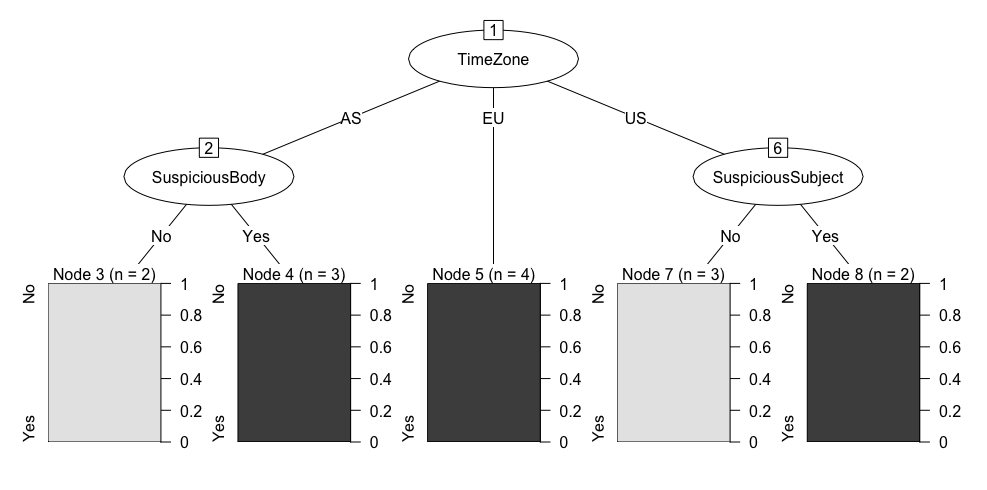
\includegraphics[scale=0.5]{RWeka_decision_tree.png}\\
The structure of both trees is the same, the R-package probably used the same algorithm as we did. The generated tree additionally shows the amount of Yes/No.
\question{}{For the source code for predictions see question b). Because the trees are the same the predictions are the same as well:\\
E-mail A = (US, US, Yes, Yes) $\Rightarrow$ Yes \\
E-mail B = (AS, AS, No, No) $\Rightarrow$ No \\
E-mail C = (EU, AS, No, Yes) $\Rightarrow$ Yes}

		\end{exercise}

		
		
\end{ukon-infie}
\end{document}
